\documentclass[runningheads]{llncs}

\usepackage[T1]{fontenc}

\usepackage{graphicx}

\usepackage{newclude}


\usepackage{tikz}
\usetikzlibrary{shapes.geometric,positioning,shapes.symbols}


\title{Modular IDE}

\author{Nils Michael Fitjar\inst{1,2}
}

\authorrunning{Nils Michael Fitjar}

\institute{Western Norway University of Applied Sciences\\
\email{798183@stud.hvl.no}
 \and
University of Bergen\\
\email{nfi005@uib.no}
}

\begin{document}
\maketitle
\begin{abstract}
This paper introduces a modular Integrated Development Environment (IDE) for experimental programming languages,
addressing limitations in traditional IDEs. While standard IDEs are crucial in software development,
their support for experimental languages is often inadequate. This project proposes a modular IDE to extend its
lifespan and enhance support for experimental languages. Analyzing the essential features of traditional IDEs and
the need for adaptability to new paradigms and tools. Magnolia, a generic programming language developed at UIB,
serves as a case study, highlighting its unique characteristics and the necessity for a specialized IDE.
The primary research question explores how modularization facilitates the design and implementation of experimental
programming languages. Specific modules or plugins tailored for experimental languages, including
Abstract Semantic Representation (ASR) Transformation, Term Algebras, MoA translation,
and Syntactic Theory Functor (STF), are outlined. These plugins will be implemented to validate the
modularized IDE's functionality, with a focus on the ASR Transformation module.

\keywords{Modularization \and IDE \and Magnolia.}
\end{abstract}

\include*{sections/000_introduction}

\include*{sections/001_background}

\include*{sections/002_research_question}

\include*{sections/003_plugins}

\include*{sections/004_implementation}

\include*{sections/005_architecture}

%% Calling C Code in Rust
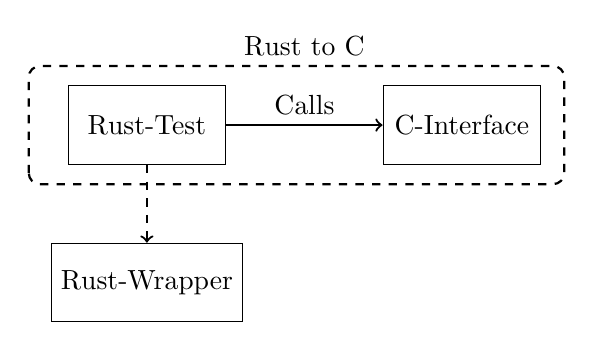
\begin{tikzpicture}
  % Nodes
  \node (RS) [rectangle, draw, minimum height=1cm, minimum width=2cm] at (0, 0) {Rust-Test};
  \node (C) [rectangle, draw, minimum height=1cm, minimum width=2cm] at (4, 0) {C-Interface};
  \node (WRAP) [rectangle, draw, minimum height=1cm, minimum width=2cm] at (0, -2) {Rust-Wrapper};
  % Arrows
  \draw[->, thick] (RS) -- (C) node[midway, above] {Calls};
  \draw[->, dashed, thick] (RS) -- (WRAP) node[midway, above] {};
  % Header
  \node (title) at (2, 1) {Rust to C};
  % Dashed lines
  \draw[dashed, thick, rounded corners] (-1.5, -0.75) rectangle (5.3, 0.75);
\end{tikzpicture}

\hfill \break %% newline

%% RS can *use* C results
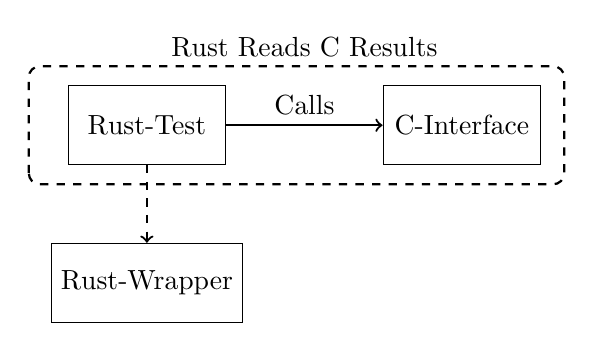
\begin{tikzpicture}
  % Nodes
  \node (RS) [rectangle, draw, minimum height=1cm, minimum width=2cm] at (0, 0) {Rust-Test};
  \node (C) [rectangle, draw, minimum height=1cm, minimum width=2cm] at (4, 0) {C-Interface};
  \node (WRAP) [rectangle, draw, minimum height=1cm, minimum width=2cm] at (0, -2) {Rust-Wrapper};
  % Arrows
  \draw[->, thick] (RS) -- (C) node[midway, above] {Calls};
  \draw[->, dashed, thick] (RS) -- (WRAP) node[midway, above] {};
  % Header
  \node (title) at (2, 1) {Rust Reads C Results};
  % Dashed lines
  \draw[dashed, thick, rounded corners] (-1.5, -0.75) rectangle (5.3, 0.75);
\end{tikzpicture}

\hfill \break %% newline

%% Converting C types to Rust types
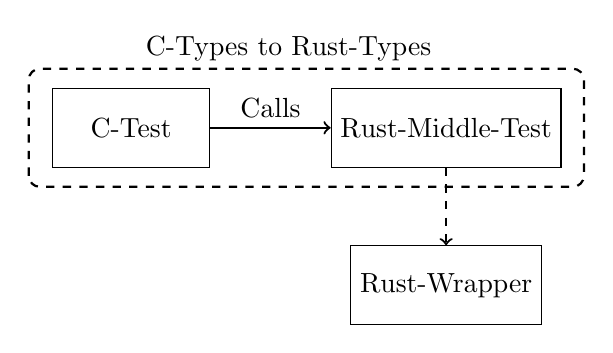
\begin{tikzpicture}
  % Nodes
  \node (C) [rectangle, draw, minimum height=1cm, minimum width=2cm] at (0, 0) {C-Test};
  \node (RS-TEST) [rectangle, draw, minimum height=1cm, minimum width=2cm] at (4, 0) {Rust-Middle-Test};
  \node (RS) [rectangle, draw, minimum height=1cm, minimum width=2cm] at (4, -2) {Rust-Wrapper};
  % Arrows
  \draw[->, thick] (C) -- (RS-TEST) node[midway, above] {Calls};
  \draw[->, dashed, thick] (RS-TEST) -- (RS) node[midway, above] {};
  % Header
  \node (title) at (2, 1) {C-Types to Rust-Types};
  % Dashed lines
  \draw[dashed, thick, rounded corners] (-1.3, -0.75) rectangle (5.75, 0.75);
\end{tikzpicture}

\hfill \break %% newline

%% Calling Rust Plugins
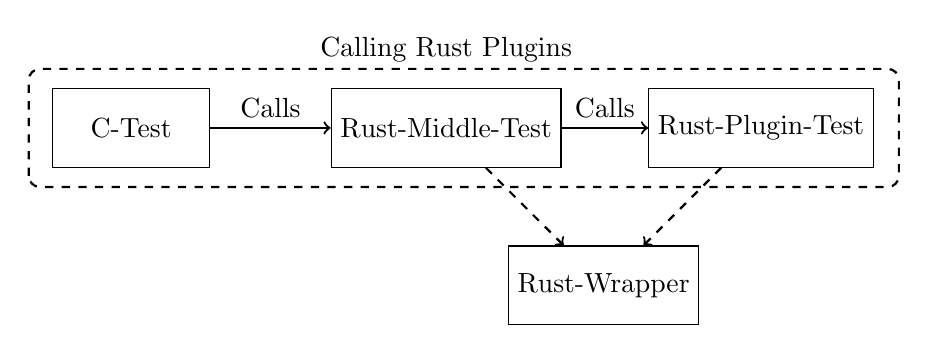
\begin{tikzpicture}
  % Nodes
  \node (C) [rectangle, draw, minimum height=1cm, minimum width=2cm] at (0, 0) {C-Test};
  \node (RS-TEST) [rectangle, draw, minimum height=1cm, minimum width=2cm] at (4, 0) {Rust-Middle-Test};
  \node (RS) [rectangle, draw, minimum height=1cm, minimum width=2cm] at (6, -2) {Rust-Wrapper};
  \node (P) [rectangle, draw, minimum height=1cm, minimum width=2cm] at (8, 0) {Rust-Plugin-Test};
  % Arrows
  \draw[->, thick] (C) -- (RS-TEST) node[midway, above] {Calls};
  \draw[->, dashed, thick] (RS-TEST) -- (RS) node[midway, above] {};
  \draw[->, dashed, thick] (P) -- (RS) node[midway, above] {};
  \draw[->, thick] (RS-TEST) -- (P) node[midway, above] {Calls};
  % Header
  \node (title) at (4, 1) {Calling Rust Plugins};
  % Dashed lines
  \draw[dashed, thick, rounded corners] (-1.3, -0.75) rectangle (9.75, 0.75);
\end{tikzpicture}

\hfill \break %% newline

%% Calling * Plugins
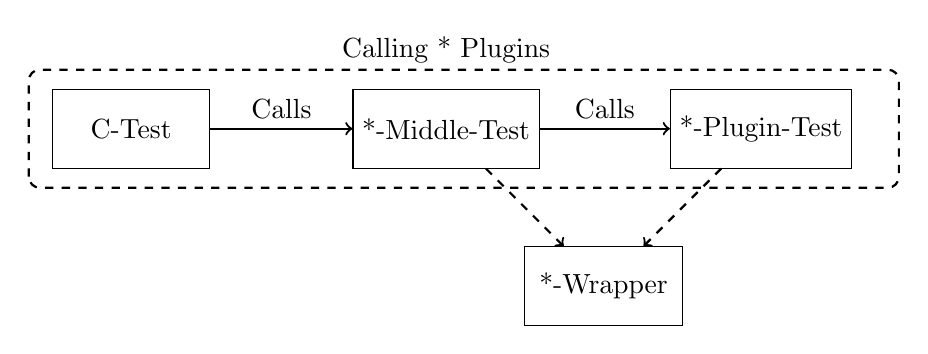
\begin{tikzpicture}
  % Nodes
  \node (C) [rectangle, draw, minimum height=1cm, minimum width=2cm] at (0, 0) {C-Test};
  \node (-TEST) [rectangle, draw, minimum height=1cm, minimum width=2cm] at (4, 0) {*-Middle-Test};
  \node (W) [rectangle, draw, minimum height=1cm, minimum width=2cm] at (6, -2) {*-Wrapper};
  \node (P) [rectangle, draw, minimum height=1cm, minimum width=2cm] at (8, 0) {*-Plugin-Test};
  % Arrows
  \draw[->, thick] (C) -- (-TEST) node[midway, above] {Calls};
  \draw[->, dashed, thick] (-TEST) -- (W) node[midway, above] {};
  \draw[->, dashed, thick] (P) -- (W) node[midway, above] {};
  \draw[->, thick] (-TEST) -- (P) node[midway, above] {Calls};
  % Header
  \node (title) at (4, 1) {Calling * Plugins};
  % Dashed lines
  \draw[dashed, thick, rounded corners] (-1.3, -0.75) rectangle (9.75, 0.75);
\end{tikzpicture}


\end{document}
